\documentclass[a4paper, 11pt, openany]{report}

% --- IMPOSTAZIONI LINGUA E FONT ---
\usepackage[utf8]{inputenc}
\usepackage[T1]{fontenc}
\usepackage{hyperref}
\usepackage{multicol}
\usepackage[italian]{babel}
\usepackage{lmodern} % Font di base pulito
\usepackage[default]{raleway} % Font sans-serif moderno per titoli
\renewcommand{\familydefault}{\sfdefault}

% --- GEOMETRIA E COLORI ---
\usepackage[margin=2.5cm]{geometry}
\usepackage{xcolor}
% Definiamo un colore principale (es. un rosso mattone o verde salvia)
\definecolor{ChefColor}{HTML}{E67E22} % Arancione scuro
\definecolor{LightBG}{HTML}{FDF2E9}   % Sfondo chiarissimo per box

% --- IMMAGINI E ICONE ---
\usepackage{graphicx}
\usepackage{wrapfig}
\usepackage{fontawesome5} % Per le icone (orologio, piatto, ecc.)

% --- FORMATTAZIONE TITOLI (NUOVO CODICE) ---
\usepackage{titlesec}

\titleformat{\chapter}[hang] % [hang] mette numero e titolo sulla stessa linea
  {\normalfont\huge\bfseries\color{ChefColor}} % Stile del testo
  {\thechapter.} % Scrive solo il numero seguito da un punto
  {1em} % Spazio tra il numero e il titolo
  {\Huge} % Dimensione del titolo

% Riduciamo anche lo spazio bianco sopra il titolo
\titlespacing*{\chapter}{0pt}{-30pt}{20pt}

% --- PACCHETTO PER INDICE LOCALE ---
\usepackage{minitoc}
% 1. Abilita la generazione dei mini-indici
\dominitoc 
% 2. Imposta l'indice locale per mostrare solo il livello 'section' (le ricette)
\setcounter{minitocdepth}{1}

% --- PACCHETTI GRAFICI PER BOX ---
\usepackage{tcolorbox}
\tcbuselibrary{skins, breakable}

% --- BOX VALORI NUTRIZIONALI ---
\newtcolorbox{boxnutrizionali}[1][]{
    colback=white, % Sfondo bianco
    colframe=gray!50, % Bordo grigio chiaro
    title={\textbf{\faChartBar\ \ Valori Nutrizionali (per porzione)}}, % Titolo
    fonttitle=\small\bfseries,
    arc=1mm,
    boxrule=0.3pt,
    coltitle=gray!20!black,
    #1
}

% =========================================================
%   DEFINIZIONE COMANDI PERSONALIZZATI PER LE RICETTE
% =========================================================

% 1. Intestazione Ricetta (Titolo + Info)
\DeclareRobustCommand{\ricetta}[5]{%
    \clearpage
    % #1 = Titolo, #2 = Tempo, #3 = Porzioni, #4 = Difficoltà, #5 = Nutrizionali
    \addcontentsline{toc}{section}{#1} 
    
    \begin{center}
        {\Huge \bfseries \color{ChefColor} #1} \\[0.5cm]
        \color{gray}
        \faClock\ \textbf{Tempo:} #2 \quad | \quad 
        \faUtensils\ \textbf{Porzioni:} #3 \quad | \quad 
        \faSignal\ \textbf{Difficoltà:} #4
    \end{center}
    
    % *** PUNTO CHIAVE: INSERIAMO MULTICOLS DENTRO IL BOX ***
    \begin{boxnutrizionali}
        \begin{multicols}{2} % SUDDIVIDE IL CONTENUTO IN 2 COLONNE
            #5
        \end{multicols}
    \end{boxnutrizionali}
    
    \vspace{0.5cm}
}
% 2. Box Ingredienti (Colonna laterale o box dedicato)
\newtcolorbox{boxingredienti}[1][]{
    colback=LightBG,
    colframe=ChefColor,
    title={\Large \faShoppingBasket\ \ Ingredienti},
    fonttitle=\bfseries,
    arc=2mm,
    boxrule=0.5pt,
    coltitle=white,
    #1
}

% 3. Ambiente Procedimento
\newenvironment{procedimento}
{
    \vspace{0.5cm}
    {\Large \bfseries \color{ChefColor} \faListUl\ \ Procedimento}
    \par\vspace{0.3cm}
    \begin{enumerate}
    \setlength\itemsep{1em} % Spazio tra i passaggi
}
{
    \end{enumerate}
}

%4. Note dello chef
\newtcolorbox{notachef}{
    colback=yellow!10!white,
    colframe=yellow!50!orange,
    title={{\faStar} \ Appunti},
    fonttitle=\bfseries,
}


% =========================================================
%   INIZIO DOCUMENTO
% =========================================================
\begin{document}

% --- COPERTINA ---
\begin{titlepage}
    \centering
    \vspace*{3cm}
    {\Huge \bfseries \color{ChefColor} I miei progressi in cucina}\\[1cm]
    {\Large \textit{Ricette di GabboAllo}}\\[2cm]
    \includegraphics[width=0.6\textwidth]{example-image-a} % Sostituisci con una tua foto
    \vfill
\end{titlepage}

% --- INDICE ---
\tableofcontents

% --- CAPITOLO 1: Antipasti ---
\chapter{Antipasti e Stuzzichini}
\minitoc


\chapter{Primi Piatti}
\minitoc

\chapter{Secondi Piatti}
\minitoc
\ricetta{Vellutata di piselli e feta}{30 min}{1 Persona}{Facile}{
        \textbf{Calorie:} 555 kcal \\
        \textbf{Proteine:} 36.6 g \\
        \textbf{Lipidi:} 31.4 g\\
        \textit{Di cui AGS:} 13.4 g \\
        \textbf{Carboidrati:} 31.6 g \\
        \textit{Di cui CHOs:} 11.6 g\\
        \textbf{Fibra:} 12.5 g\\
        \textbf{Sodio:} 0.5 g
}

% IL CONTENUTO DELLA RICETTA (Ingredienti e Procedimento)
\begin{minipage}[t]{0.35\textwidth}
    \begin{boxingredienti}
        \begin{itemize}
            \item 250g piselli freschi o surgelati
            \item 100g feta
            \item 30g cipolla
            \item 10g olio EVO
        \end{itemize}
    \end{boxingredienti}
    
    \vspace{0.5cm}
    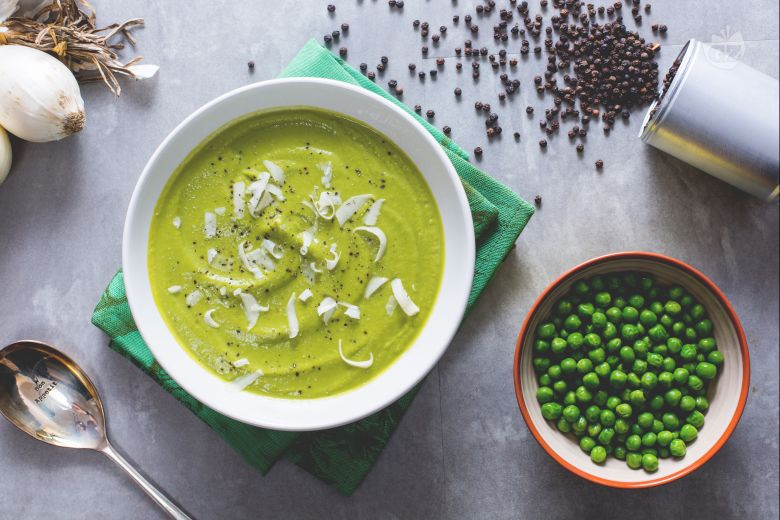
\includegraphics[width=\textwidth, keepaspectratio]{Vellutata.jpg}
\end{minipage}
\hfill 
\begin{minipage}{0.60\textwidth}
    \begin{procedimento}
        \item Mettere un pentolino d'acqua a bollire.
        \item In un'altra pentola far soffriggere la cipolla e aggiungere i piselli quando è pronta. 
        \item Dopo \textbf{5 minuti} di cottura versare l'acqua bollente insieme ai piselli e far andare il tutto a fiamma alta con il coperchio per far evaporare l'acqua (se in eccesso).
        \item Dopo \textbf{20 minuti} di cottura spegnere il fuoco e frullare i piselli con il minipimer aggiungendo la feta durante la frullatura. \textit{Se l'acqua è ancora troppa scolarne un po'.}
        \item Versare la vellutata nel piatto.
    \end{procedimento}
\end{minipage}

\begin{notachef}
Il primo tentativo è andato bene: la vellutata era buona ma decisamente troppa (ho usato più di 300g di piselli) e si sentiva tanto la feta (ne ho usata una intera).\\
Per evitare di fare casini quando si frulla travasa volta per volta un po' di piselli e feta dentro ad un contenitore cilindrico e non usare la pentola. 
\end{notachef}

\end{document}